\documentclass{article}
\usepackage[margin=1in]{geometry}
\usepackage{microtype}
\usepackage{setspace}
\usepackage{amsmath}
\usepackage{parskip}
\usepackage{amssymb}
\usepackage{graphicx}

\graphicspath{{../public/}}

\parskip=4ex
\date{}
\author{}

\title{10.3 The Dot Product}

\begin{document}
  \maketitle
  \textbf{Definition}\\
  If $  \vec{a} = <a_1, a_2, a_3> $ and $ \vec{b} = <b_1, _2, b_3> $ then the dot product of $ \vec{a} $ and $ \vec{b} $ is the number $ \vec{a} \cdot \vec{b} $ given by $ \vec{a} \cdot \vec{b} $ given by $ \vec{a} \cdot \vec{b} = a_1b_1+a_2b_2+a_3b_3 $. While for 2 dimensional vectors, $ <a_1, a_2> \cdot <b_1, b_2>= a_1b_1+a_2b_2 $

  \textbf{Ex 1. Find the dot product}
  \[
    \begin{gathered}
       <2, 4>\cdot <3, -1> = 2(3)+4(-1)=6-4=\boxed{2}\\
       < -1, 7, 4> \cdot <6, 2, -\frac{1}{2}> = -1(6) + 7(2) + 4( -\frac{1}{2}) = \boxed{6}\\
       ( \vec{i} + 2 \vec{j} - 3 \vec{k}) \cdot (2 \vec{j} - \vec{k})=1(0)+2(2)+(-3)(-1)=\boxed{7}
    \end{gathered}
  \]

  \textbf{Properties}\\
  If $ \vec{a}, \vec{b} $ and $ \vec{c} $ are 3-dimensional vectors, and c is a scalar, then

  \[
    \begin{gathered}
     \vec{a} \cdot \vec{a} = | \vec{a} |^2\\
     \vec{a} \cdot \vec{b} = \vec{b} \cdot \vec{a}\\
     \vec{a} \cdot ( \vec{b} + \vec{c}) = \vec{a} \cdot \vec{b} + \vec{a} \cdot \vec{c}\\
     (c \vec{a}) \cdot \vec{b} = c( \vec{a} \cdot \vec{b}) = \vec{a} \cdot (c \vec{b})\\
     \vec{0} \cdot \vec{a} = 0
    \end{gathered}
  \]
  \textbf{Angle Between 2 Vectors}\\
  $ 0 \le \theta \le \pi $. If $\vec{a}$ and $\vec{b}$ are parallel, then $ \theta = 0 $ or $ \theta = \pi $

  \textbf{Theorem}\\
  If $ \theta $ is the angle between the vectors $ \vec{a} $ and $ \vec{b} $, then
  \[
      \vec{a} \cdot \vec{b}=| \vec{a} |\cdot | \vec{b} | \cdot \cos{\theta}
  \]

  \textbf{Ex 2}\\
  If the vectors $ \vec{a} $ and $ \vec{b} $ have lengths 4 and 6, and the angle between them is $ \frac{\pi}{3} $, find $ \vec{a} \cdot \vec{b} $.
  \[
    \begin{aligned}
      | \vec{a} | = 4, | \vec{b} | = 6\\
      \vec{a} \cdot \vec{b} = 4(6) \cos{ \frac{\pi}{3}} = 24( \frac{1}{2}) = \boxed{12}
    \end{aligned}
  \]

  \textbf{Ex 3}\\
  Find the angle between the vectors $ \vec{a} = < 2, 2, -1> \& \vec{b}=< 5, -3, 2> $.
  \[
    \begin{gathered}
    \vec{a} \cdot  \vec{b} = 2(5)+2(-3)+(-1)(2)=2\\
    ~\\
    | \vec{a} | = \sqrt{(2)^{2} + (2)^{2} + (-1)^{2}} = \sqrt{9} = 3\\
    ~\\
    | \vec{b} | = \sqrt{(5)^{2}+(-3)^{2} + (2)^{2}   } = \sqrt{38}\\
    ~\\
    \vec{a} \cdot \vec{b}=| \vec{a} | | \vec{b} | \cos{\theta}\\
    \cos{\theta}= \frac{\vec{a}\cdot \vec{b}}{| \vec{a} || \vec{b} |}= \frac{2}{3\sqrt{38} } \\
    ~\\
    \theta=\cos^{-1}{\frac{2}{3\sqrt{38} }}\approx \boxed{1.46}
    \end{gathered}
  \]

  \textbf{Definition}\\
  Two nonzero vectors $ \vec{a} ~\& ~\vec{b} $ are called \underline{perpendicular} or \underline{orthogonal} if the angle between them is $ \theta=\frac{\pi}{2} $.
  
  \textbf{Ex 4}\\
  Show that $ 2\vec{i}+2\vec{j}-\vec{k} $ is perpendicular to $ 5\vec{i}-4\vec{j}+2\vec{k} $.
  
  \[
    \begin{gathered}
      (2\vec{i}+2\vec{j}-\vec{k}) \cdot (5\vec{i}-4\vec{4}+2\vec{k})\\
      2(5) + 2(-4) + (-1)(2)\\
      10-8-2=0\\
      \text{Thus, the vectors are perpendicular.}
    \end{gathered}
  \]

  \textbf{Intepretation of Dot Product}
  \[
    \begin{gathered}  
  0\le\theta<\frac{\pi}{2}\\
  \vec{a}\cdot \vec{b}>0, \text{since} \cos{\theta}>0  
    \end{gathered}
  \]
  \[
    \begin{gathered}
    \theta=\frac{\pi}{2} \\
    \vec{a}\cdot \vec{b}=0, \text{since} \cos{\frac{pi}{2}=0 }
    \end{gathered}
  \]
  \textbf{Theorem}\\
  Two vectors $ \vec{a} ~\& ~\vec{b} $ are orthogonal if and only if $ \vec{a} \cdot \vec{b} = 0$. 

  If $ \theta = 0 $, then $ \vec{ a } \cdot \vec{ b }   $ = $ | \vec{ a }  |  | \vec{ b }  |$ since $ \cos{0} = 1$.\\
  If $ \theta = 0 $, then $ \vec{ a } \cdot \vec{ b }   $ = $ -| \vec{ a }  |  | \vec{ b }  |$ since $ \cos{0} = -1$.

  \textbf{Projections}\\
  Suppouse we have two vectors, $ a ~\&~ b $. The projection of $ b $  onto another vector, $ a $ can be thought of the shadow of vector $ b $ that overlaps vector $ a $ from vertices $ P ~\&~ S $ or vector $ \vec{PS} $. So then the vector $ \vec{PS} $ is the vector projection of $ b $ onto $ a $ or denoted as comp$_{a}b$. 

  \begin{center}
    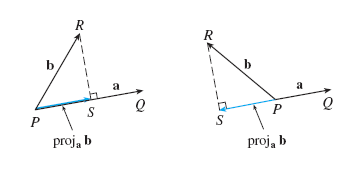
\includegraphics[width=8cm]{vector_projection}
  \end{center}

  There is another type of projection called a scalar projection, which is the signed magnitude of comp$_{a}b$. 

  \[
    \begin{gathered}
      \text{Scalar Projection of } b \text{ onto } a\\
      \text{comp}_{a}b = \frac{a \cdot b}{| a |}\\
      ~\\ 
    \text{Vector Projection of } b \text{ onto } a\\
    \text{proj}_{a}b = \frac{a \cdot b}{| a |} \cdot \frac{a}{| a |}
    \end{gathered}
  \]

  Suppouse we have two vectors $ \vec{a} ~\&~ \vec{b} $. The vector projection of $ \vec{b} $ onto $ \vec{a} $ is proj$ _{\vec{a}}\vec{b}  $. While the scalar projetion of $ \vec{b} $ onto $ \vec{a} $ is comp$ _{\vec{a}}\vec{b}$. Also note that the composition formula is derived from the dot product formula like so
  \[
    \begin{gathered}
     \vec{a} \cdot  \vec{b} = | \vec{a} | | \vec{b} | \cos{\theta}\\
     ~\\
     \frac{\vec{a} \cdot \vec{b}}{| \vec{a} |} = | \vec{b} | \cos{\theta}
    \end{gathered}
  \]

\textbf{Ex 5}\\
Find the scalar and vector projects of $  \vec{ b } = < 1, 1, 2>   $ onto $ \vec{ a } = < -2, 3, 1>   $   

\[
  \begin{aligned}
  &	\text{comp} _{ \vec{ a } }\vec{ b } = \frac{ -2(1) + 3(1) + 1(2)}{ \sqrt{ (-2) ^{2} + (3)^2 + (1)^2  }} = \boxed{ \frac{ 3 }{ \sqrt{ 14 }   } }
  \end{aligned}
\]

\textbf{Calculating Work}\\
The work done bt a constant force $ f $  in moving an object through a distance $ d $  is $ W=FD $.\\
Suppouse the constant force is a vector $ \vec{ F }  $ pointing in a direction different from the displacement vector $\vec{ D }$.

If the force moves the object from points $ P \to Q $ along a straight line ($ \theta = 0,~cos(\theta)=1 $ ), then the work can be calculated like so
\[
  \begin{aligned}
  & W= ( | \vec{ F }  | \cos{\theta})\\ 
  & W = | \vec{ F }  | \vec{ D } \cos{ \theta}\\
  & W = \vec{ F } \cdot \vec{ D }  
  \end{aligned}
\]

\textbf{Ex 6}\\
A force is given by a vector $ \vec{ F } = 3 \vec{ i } + 4 \vec{ j } + 5 \vec{ k } $ and moves a particle from the point $ P (2,1,0) $ to the point $ Q(4,6,2) $, find the work done.
\[
  \begin{aligned}
  &	\vec{ D } = \vec{ PQ } = < 4-2, 6-1, 2-0>\\
  & = < 2, 5, 2>\\
  ~\\
  & W = \vec{ F } \cdot \vec{ D } = 3(2) + 4(5) + 5(2) \\
  & = 6 + 20 + 10\\
  & = \boxed{30}
  \end{aligned}
\]

 
\end{document}
